\chapter{Arquitectura del Sistema}

La arquitectura del sistema Gestión de Comandas adopta el modelo
\textbf{BaaS (Backend as a Service)}. En este enfoque, el cliente móvil
consume directamente los servicios proporcionados por Supabase sin la
necesidad de un backend intermedio personalizado.

Supabase provee servicios administrados de base de datos, autenticación,
almacenamiento de archivos y sincronización en tiempo real, lo cual reduce
la complejidad de infraestructura y permite enfocar el desarrollo en la
lógica de negocio y la experiencia de usuario.

\section{Diagrama de Contexto}

El diagrama de contexto muestra la interacción general entre los actores
del sistema (mesero, administrador y cliente) y los servicios principales
utilizados en la solución. Se observa cómo la aplicación móvil y la carta
digital web se comunican directamente con Supabase mediante protocolos
REST, WebSocket y mecanismos de autenticación basados en JWT.

\begin{figure}[H]
\centering
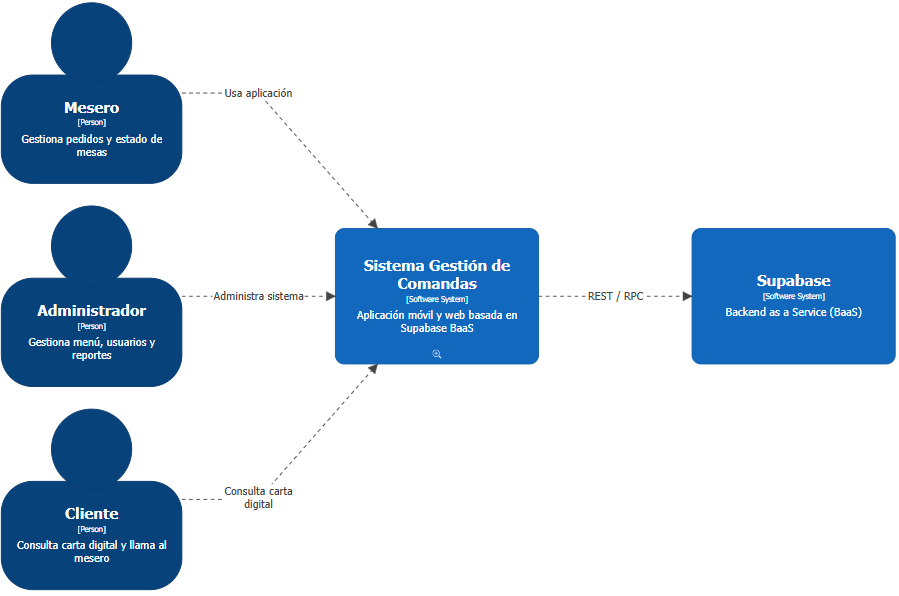
\includegraphics[width=0.95\textwidth]{img/context.png}
\caption{Diagrama de Contexto del sistema Gestión de Comandas basado en modelo BaaS}
\end{figure}

En este nivel se identifican los usuarios del sistema y los sistemas externos
con los que interactúa la solución. El cliente móvil implementado en React
Native consume directamente los servicios de Supabase PostgreSQL, Supabase
Auth, Supabase Storage y Supabase Realtime. Asimismo, la carta digital
accesible mediante navegador web permite a los clientes consultar el menú
y solicitar atención sin necesidad de autenticación tradicional.

\section{Diagrama de Contenedores}

El diagrama de contenedores describe los bloques principales que componen
la solución y cómo estos se comunican entre sí. Se distinguen claramente
los contenedores del cliente móvil, las rutas web públicas y los servicios
gestionados por Supabase.

\begin{figure}[H]
\centering
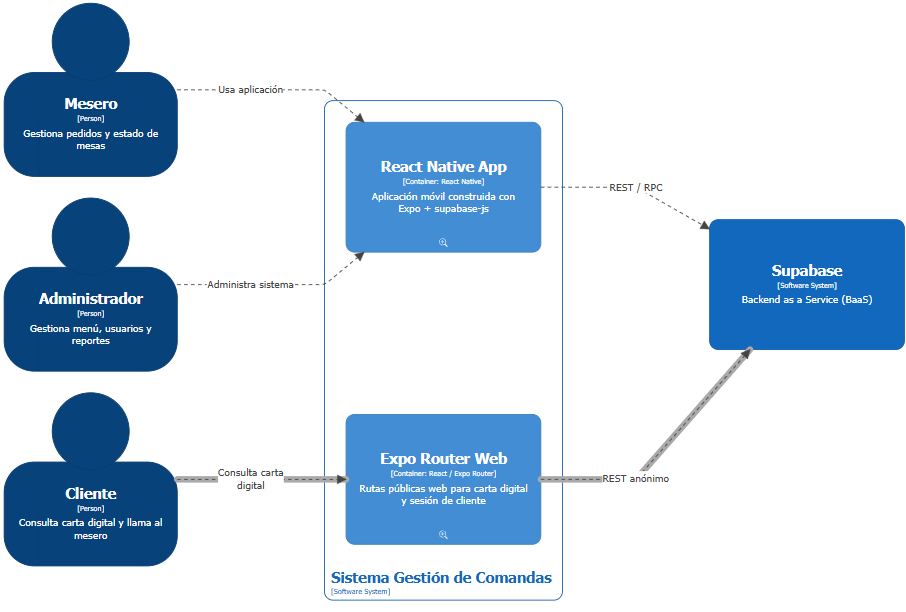
\includegraphics[width=0.95\textwidth]{img/containers.png}
\caption{Diagrama de Contenedores del sistema utilizando Supabase como Backend as a Service}
\end{figure}

La aplicación móvil desarrollada con React Native y Expo se conecta
directamente a Supabase mediante el SDK oficial supabase-js. Este cliente
permite realizar consultas a la base de datos, autenticación de usuarios,
subida de archivos y suscripción a eventos en tiempo real.

Por otro lado, Expo Router permite exponer rutas web públicas que facilitan
la visualización de la carta digital y la sesión del cliente en mesa mediante
el uso de códigos QR. Estas rutas utilizan acceso anónimo controlado mediante
las políticas de seguridad Row Level Security (RLS).

Supabase actúa como proveedor de Backend as a Service ofreciendo:

\begin{itemize}
\item Base de datos PostgreSQL con funciones SQL y políticas RLS.
\item Servicio de autenticación basado en JWT y roles.
\item Almacenamiento de imágenes del menú mediante Storage con acceso público.
\item Canales de comunicación en tiempo real mediante WebSocket.
\end{itemize}

\section{Diagrama de Componentes — Funcionalidades Clave}

\subsection{Componentes de la aplicación móvil}

El siguiente diagrama muestra los componentes principales de la aplicación
móvil utilizada por el mesero y el administrador. Estos componentes permiten
gestionar pedidos, visualizar el estado de mesas, administrar el menú y
consultar reportes financieros.

\begin{figure}[H]
\centering
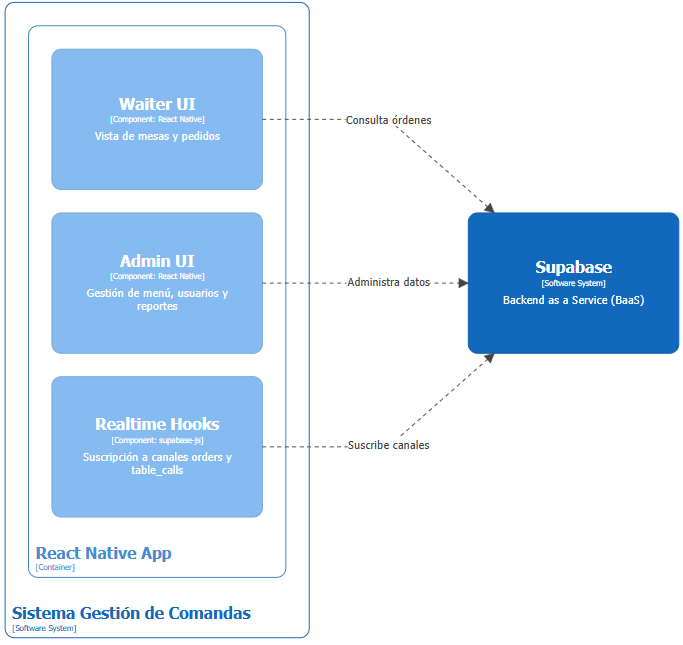
\includegraphics[width=0.95\textwidth]{img/components-mobile.png}
\caption{Componentes principales de la aplicación React Native}
\end{figure}

Los componentes Waiter UI y Admin UI representan las interfaces de usuario
según el rol autenticado. El módulo Realtime Hooks permite la suscripción a
los canales de Supabase Realtime para actualizar el estado de las mesas y
los pedidos sin necesidad de recargar la aplicación.

\subsection{Componentes de rutas web públicas}

El siguiente diagrama muestra los componentes asociados a la carta digital
y la sesión del cliente en mesa. Estas funcionalidades permiten que el cliente
visualice el menú mediante un código QR y pueda solicitar atención al mesero.

\begin{figure}[H]
\centering
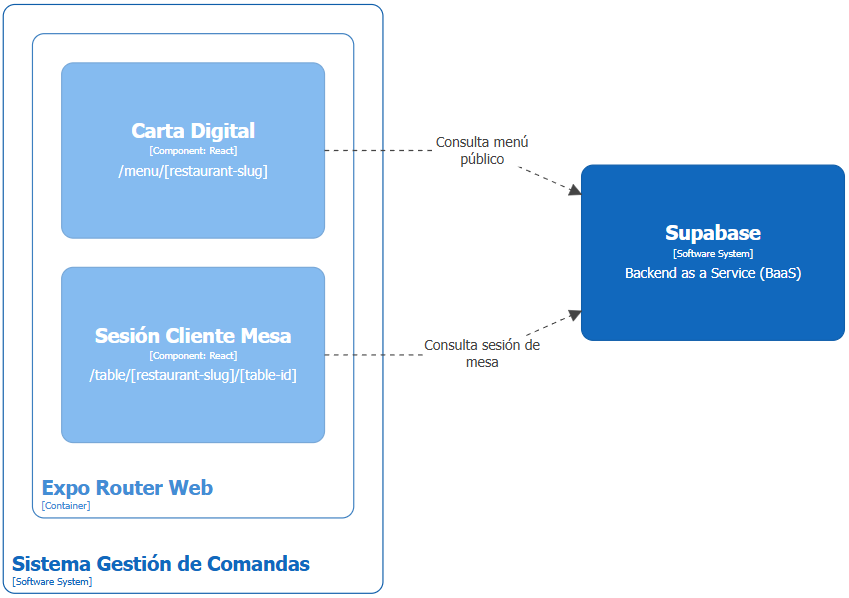
\includegraphics[width=0.95\textwidth]{img/components-web.png}
\caption{Componentes de la carta digital y sesión de cliente en mesa}
\end{figure}

Las rutas públicas permiten acceder al menú del restaurante utilizando un
identificador único (slug). La sesión de mesa permite identificar la mesa
desde la cual el cliente solicita atención, registrando eventos en la base
de datos que son posteriormente consumidos por la aplicación del mesero en
tiempo real.


\subsection{Contexto de Supabase}

El siguiente diagrama muestra cómo la aplicación cliente interactúa con los
servicios ofrecidos por Supabase dentro del modelo Backend as a Service (BaaS).
En este enfoque, el cliente móvil y las rutas web públicas consumen directamente
los servicios de autenticación, base de datos, almacenamiento y comunicación en
tiempo real sin necesidad de un backend intermedio personalizado.

\begin{figure}[H]
\centering
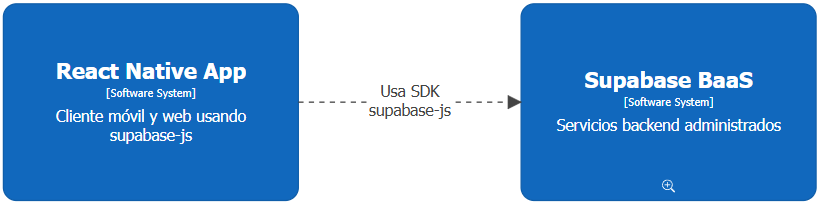
\includegraphics[width=0.9\textwidth]{img/supabase-context.png}
\caption{Relación entre la aplicación cliente y los servicios de Supabase}
\end{figure}

Supabase proporciona un conjunto de servicios integrados que permiten reducir
la complejidad de infraestructura. El SDK supabase-js facilita la conexión desde
la aplicación React Native hacia PostgreSQL, Auth, Storage y Realtime utilizando
protocolos seguros basados en JWT y WebSocket.


\subsection{Contenedores de Supabase}

El diagrama de contenedores presenta los servicios principales que conforman el
Backend as a Service utilizado en el sistema. Cada contenedor cumple una función
específica dentro de la arquitectura, permitiendo desacoplar responsabilidades
y facilitar la escalabilidad del sistema.

\begin{figure}[H]
\centering
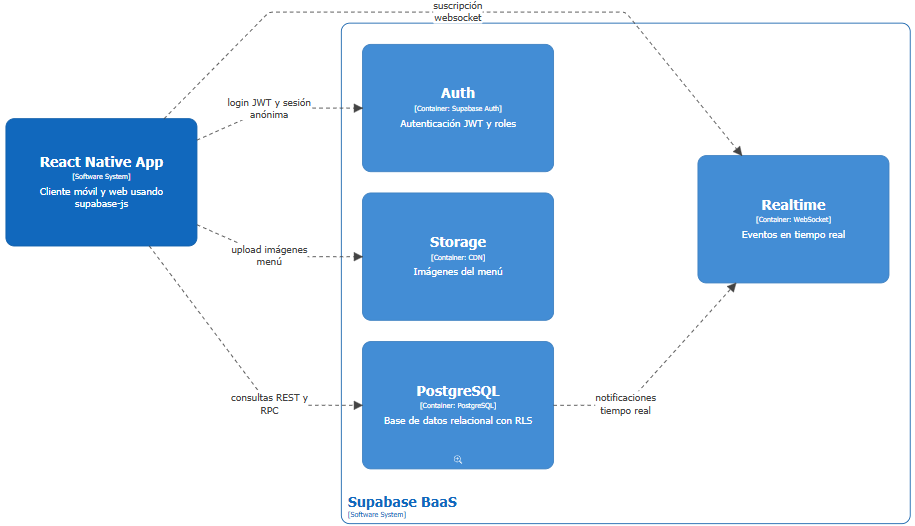
\includegraphics[width=0.9\textwidth]{img/supabase-containers.png}
\caption{Contenedores principales del entorno Supabase}
\end{figure}

El contenedor PostgreSQL almacena la información relacionada con usuarios,
mesas, pedidos, gastos y reportes. El servicio Auth permite gestionar sesiones
de usuario mediante tokens JWT, soportando autenticación tradicional y sesiones
anónimas utilizadas por la carta digital.

El servicio Storage permite almacenar imágenes de los productos del menú, las
cuales son accesibles mediante URLs públicas optimizadas mediante CDN. Por otro
lado, el servicio Realtime permite mantener sincronizados los estados de pedidos
y llamadas de clientes mediante WebSockets.


\subsection{Componentes de la Base de Datos}

El siguiente diagrama describe los componentes internos de la base de datos
implementada en Supabase. Se incluyen las tablas principales, sus relaciones
lógicas y las funciones SQL utilizadas para generar reportes financieros y
análisis de ventas.

\begin{figure}[H]
\centering
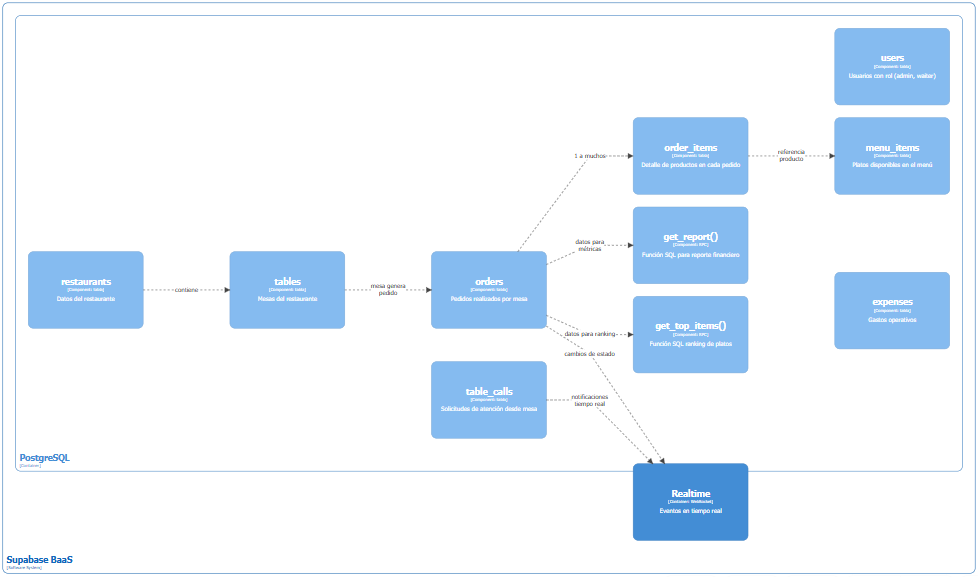
\includegraphics[width=0.95\textwidth]{img/supabase-components.png}
\caption{Componentes internos del esquema de base de datos en Supabase}
\end{figure}

La tabla \texttt{users} almacena los usuarios del sistema con sus respectivos
roles. La tabla \texttt{restaurants} permite gestionar
la información del restaurante, mientras que la tabla \texttt{tables} representa
las mesas disponibles en el establecimiento.

Las tablas \texttt{orders} y \texttt{order\_items} almacenan la información de
los pedidos realizados, manteniendo consistencia histórica de precios mediante
snapshots de los productos seleccionados. La tabla \texttt{expenses} permite
registrar los gastos operativos necesarios para el cálculo de métricas financieras.

\subsection{Vista de Estado de Mesas (Mesero)}

La pantalla principal del mesero muestra en tiempo real el estado de cada
mesa asignada. Esta funcionalidad se basa en la suscripción al canal
\texttt{orders} de Supabase Realtime, permitiendo actualizar los estados
de los pedidos sin necesidad de recargar la aplicación.

Adicionalmente, la aplicación escucha el canal \texttt{table\_calls}, el cual
permite detectar cuando un cliente solicita atención desde su mesa mediante
la carta digital.

\begin{center}
\begin{tabular}{ll}
  \toprule
  \textbf{Estado visual} & \textbf{Condición en DB} \\
  \midrule
  Libre                  & Sin orden activa para esa mesa en la fecha actual \\
  Pendiente              & \texttt{status = 'pending'} \\
  Listo para entregar    & \texttt{status = 'ready'} \\
  Entregado              & \texttt{status = 'delivered'} \\
  Cliente llama          & Registro en \texttt{table\_calls} con \texttt{attended = false} \\
  \bottomrule
\end{tabular}
\end{center}

Este mecanismo permite mantener sincronizados los estados entre múltiples
dispositivos conectados simultáneamente, asegurando consistencia en la
información mostrada al personal del restaurante.